\chapter[Forschungsfrage 2]{Welche wirtschaftlichen Vorteile hat der Einsatz von Container auf den Prozess des automatisierten \enquote{Deployments}?} \label{ff2}
In diesem Kapitel ...

\section{Grundlagen: Definieren der Begrifflichkeiten zur Forschungsfrage zwei}
Dieses Teilkapitel soll grundlegende Begrifflichkeiten, die im weiteren Verlauf dieser Arbeit verwendet werden, definieren, um so eine einheitliche Terminologie der Begriffe zu entwickeln. Dadurch wird ein gemeinsames Verständnis erzeugt.

\paragraph{Geschäftsprozessanalyse}
Der Begriff \enquote{Geschäftsprozess} beschreibt eine zusammenhängende Folge von Aufgaben beziehungsweise Tätigkeiten, die in einem Unternehmen abgeschlossen werden, um die Unternehmens-/Organisationsziele zu erreichen. Die Analyse untersucht schlussendlich dieselben Sachverhalte, wie auch die klassischen Ansätze der Organisationslehre. \autocite[vgl.][S.\,5]{staud_geschaftsprozessanalyse_2006} Diese sind klassisch die Effizienzsteigerung und die Einsparung. Dabei werden die zu leistenden Tätigkeiten, Aufgaben und Arbeitsabläufe auf die genannten Ansätze optimiert. Im Vergleich zur klassischen Optimierung steht bei der Geschäftsprozessanalyse eine andere Perspektive im Fokus. Hier werden die \enquote{längere(n) zusammenhängende(n) Folgen von Tätigkeiten, die zur Erledigung einer größeren Aufgabe nötig sind}\autocite[][S.\,5]{staud_geschaftsprozessanalyse_2006}, betrachtet. Damit ist der gesamte Ablauf eines Prozesses als Ausgangspunkt der Analyse zu betrachten und nicht mehr nur einzelne Tätigkeiten und Stellen.
\par 
Um das weitere Verständnis der Begrifflichkeiten zu fördern, werden folgende Begriffe definiert\autocite[vgl.][S.\,4-5]{staud_geschaftsprozessanalyse_2006}: Aufgaben und deren Eigenschaften, Aufgabenfolgen und Funktionen. Aufgaben sind Teilarbeitspakete einer Tätigkeit, die auf unterschiedlichen Ebenen betrachtet werden können. Die kleinste Einheit einer Aufgabe ist die Elementaraufgabe, die nicht weiter teilbar ist. Wichtig ist, dass Aufgaben teilbar und wieder zusammenfassbar sind, so wird eine unterschiedliche Aggregationsstufe erreicht. Das Problem der Aggregation ist, dass die Modelliererin, geprägt durch ihre Wahrnehmung, die Ebene der Betrachtung einer Aufgabe/Tätigkeit subjektiviert und so das Ergebnis stark beeinflusst wird -- so auch die Länge der Geschäftsprozesse. Die sequenzielle Folge von Aufgaben entsteht durch die Erstellung eines Vorgangs, der eine Abfolge von Tätigkeiten zur Realisierung von Aufgaben beschreibt. Schließlich wird ein Geschäftsprozess von \cite{staud_geschaftsprozessanalyse_2006} definiert als: \enquote{[...] besteht aus einer zusammenhängenden abgeschlossenen Folge von Tätigkeiten, die zur Erfüllung einer betrieblichen Aufgabe notwendig sind. Die Tätigkeiten werden von Aufgabenträgern in organisatorischen Einheiten unter Nutzung der benötigten Produktionsfaktoren geleistet. Unterstützt wird die Abwicklung der Geschäftsprozesse durch das Informations- und Kommunikationssystem IKS des Unternehmens.}\autocite[][S.\,9]{staud_geschaftsprozessanalyse_2006} Eine weitere Definition charakterisiert den Geschäftsprozess als \enquote{[...] eine zielgerichtete, zeitlich logische Abfolge von Aufgaben, die arbeitsteilig von mehreren Organisationen oder Organisationseinheiten unter Nutzung von Informations- und Kommunikationstechnologien ausgeführt werden können. Er dient der Erstellung von Leistungen entsprechend den vorgegebenen, aus der Unternehmensstrategie abgeleiteten Prozesszielen. Ein Geschäftsprozess kann formal auf unterschiedlichen Detaillierungsebenen und aus mehreren Sichten beschrieben werden.}\autocite[][S.\,41]{gadatsch_grundkurs_2010} Die zweite Definition wird in dieser Arbeit verwendet, denn sie stellt die Unternehmensstrategie als zentralen Messfaktor in den Mittelpunkt. Werden alle Geschäftsprozesse linear kombiniert, entsteht die Darstellung der Wertschöpfungskette eines Unternehmens. Deswegen gibt es nur systemrelevante Geschäftsprozesse in einem Unternehmen. Sie können noch Optimierungspotential enthalten, jedoch sind sie nie unnötig oder nicht brauchbar. Ein Geschäftsprozess wird an dem Kunden orientiert. Es wird zwischen Kern- und unterstützenden Prozessen unterschieden: bei Kernprozessen handelt es sich um die Hauptleistung eines Unternehmens, wie die Produktion eines Autos bei einem Autohersteller. Die Unterteilung in Kern- und unterstützende Prozesse beschreibt dabei nicht die Wichtigkeit dieser; es ist also keine Einteilung in weniger wichtig und wichtig vorzunehmen.\autocite[vgl.][S.\,11]{staud_geschaftsprozessanalyse_2006} \par

Geschäftsprozesse haben verschiedene Eigenschaften, wie der Automatisierungsgrad, die Datenintegration und die Prozessintegration. Der Automatisierungsgrad beschreibt wie groß der Anteil der Aufgabenerfüllung ist, welcher dunkel, d.\,h. ohne menschliche Interaktion, bewältigt werden kann. Die Datenintegration ist ein wichtiger Bestandteil bei Optimierungsvorhaben, denn sie sollte bei 100 Prozent liegen, um Inkonsistenzen der Daten auszuschließen. Bei weniger als 100 Prozent entwickeln sich Parallelwelten im Unternehmen. Ist ein Geschäftsprozess über viele verschiedenen traditionelle Organisationsbereiche aufgespannt, so ist seine Prozessintegration hoch. Gibt es Organisationsbrüche, d.\,h. wird ein Prozess aktiv an einer beteiligten Abteilung vorbeigeführt, muss die Notwendigkeit dieser Maßnahme bei der Optimierung überprüft werden. Zu den Komponenten der Geschäftsobjekte: Je nach Ziel der Untersuchung können beziehungsweise sind viele Komponenten beteiligt. Die \ac{BWL} beschränkt diese auf die formellen Strukturen einer Organisation und auf das Handeln der Beteiligten, das unmittelbar Einfluss auf den Geschäftsprozess hat.\autocite[vgl.][S.\,15]{staud_geschaftsprozessanalyse_2006} \par

Ziel der Geschäftsprozessanalyse ist es, eine Ist-Analyse des Prozesses durchzuführen, um so eine Bestandsaufnahme vorhalten zu können, und eine Optimierung dieses, die die Beseitigung von Schwachstellen zur Folge hat. Diese werden bei der Ist-Analyse entdeckt. Einschränkend zu erwähnen ist, dass die Methodik der Geschäftsprozessanalyse nicht genau definiert ist, da die Identifikation (Detaillierungsgrad) und Abgrenzung (Länge) der Prozesse subjektiv beeinflusst wird. Das Modell der \ac{EPK} ist eine mögliche Methodik, um Geschäftsprozesse zu analysieren und zu beschreiben.\autocite[vgl.][S.\,59]{staud_geschaftsprozessanalyse_2006} \ac{EPK} ist ein Vorgehensmodell zur sichten-orientierten Modellierung von Geschäftsprozessen, dabei wird ein Prozess und seine dazugehörenden Funktionen in einer zeitlich-logischen Abfolge illustriert.\autocite[vgl.][S.\,4]{scheer_objektorientierte_1997} Die Kontrollflusssteuerung zwischen den einzelnen Funktionen eines Geschäftsprozess werden über Geschäftsregeln gesteuert. Diese beinhalten folgende Konstrukte: Ereignis, Bedingung und Funktion/Methode/Aktion. Entscheidungen werden über die verfügbaren Verknüpfungsfunktionen modelliert:\autocite[vgl.][S.\,4]{scheer_objektorientierte_1997} \textit{AND}-, \textit{OR}- und \textit{XOR}-Verknüpfung\footnote{Hier wird an die gängige Schreibweise der Logikgatter angeknüpft.}. Des Weiteren gibt es eine andere Methodik, die in einem Standard, \ac{BPMN} Version 2.0 \autocite{object_management_group_omg_business_2011} definiert ist, die Geschäftsprozesse modelliert. Außerdem wurde dieser Standard in der Norm ISO/IEC 19510 verankert.\autocite{ict1_information_2020} Im Gegensatz zur \ac{EPK} fokussiert sich \ac{BPMN} rein auf die Modellierung eines Prozesses und nicht auf folgende Strukturen: Prozesslandschaft, Aufbauorganisation, Daten, Strategie, Geschäftsregeln und IT-Landschaft.\autocite[vgl.][S.\,28]{freund_praxishandbuch_2017} Es gibt eine Software-Lösung für \ac{BPMN}, die in der \ac{SVI} eingesetzt wird und später die erste Container-Applikation für den neuen \enquote{Deployment}-Prozess ist.

\paragraph{\enquote{Business Case}}\label{sec:businessCase}
In diesem Teilkapitel werden der Aufbau eines Geschäftsszenarios und die grundsätzliche Methodik erläutert, da eine tiefgreifende, ausführliche Beschreibung des gesamten Themenkomplexes die Notwendigkeit für diese Arbeit überschreitet. Eine vollumfängliche Betrachtung eines \enquote{Business Case} kann eine eigene Bachelor-Thesis darstellen. \par
Die Erstellung eines Geschäftsvorfalls (engl. \enquote{Business Case}) ist für das Unternehmen bei der Betrachtung eines Projekts von elementarer Bedeutung. Ohne die Erstellung dieses könnten folgende Probleme mit hoher Wahrscheinlichkeit auftreten\autocite[][S.\,4]{herman_is_2009}: 
\begin{itemize}
	\item \enquote{The organization wastes valuable resources on projects that don't help the organization achieve its objectives. This leaves fewer resources available for more valuable projects.
	\item The organization has no clear basis to prioritize projects, for establishing what is important. Without a Business Case—and some organization-wide agreed measure of “value”—there is no	means of determining which projects are important, and which are less so.
	\item There is likely to be disappointment after the completion of the
	project, as the stakeholders wonder why the project is not giving the great results they imagined [...].
	\item No target is established for why the project's deliverables are
	being created—other than the meeting of technical specifications.
	\item The organization has no opportunity to improve its project management maturity. One key learning from each project should be: “how well did the resource usage support the organization's goals?”}
\end{itemize}
Grundsätzlich ist ein Geschäftsszenario eine betriebswirtschaftliche Beurteilung einer Investition. Dabei werden Kosten und Nutzen dieser nach einer zuvor definierten Methodik gemessen, beurteilt und dokumentiert. Am Ende eines \enquote{Business Case} entsteht eine, mit Informationen begründete, Aussage über die Investition -- ist diese rentabel? Das Geschäftsszenario soll für jedes Projekt eines Unternehmens erstellt werden. Dabei soll mit diesem der Mitteleinsatz gegenüber den Führungskräften beziehungsweise der Geschäftsführung gerechtfertigt werden. Bestandteile des \enquote{Business Case} sind somit: rein monetäre Größen und nicht-monetäre Aspekte (meist Abwägungen \enquote{hinsichtlich Risikoadressierung und Strategieorientierung in Verbindung mit den jeweiligen Optionen und deren wirtschaftlicher Vorteilhaftigkeit}\autocite[][S.\,12]{brugger_it_2009}). Es entsteht eine ganzheitliche Dokumentation aller entscheidungsrelevanter Sachverhalte: \enquote{Ein Business Case fasst alle entscheidungsrelevanten Aspekte eines geplanten Vorhabens mit dem Ziel zusammen, die wirtschaftliche Vorteilhaftigkeit und strategische Konformität des Gesamtprojekts aufzuzeigen und eine abschließende Management-Entscheidung über dessen Ausführung zu ermöglichen.}\autocite[][S.\,13]{brugger_it_2009} Abzugrenzen ist dieser Begriff von dem \enquote{Business Plan}: er basiert auf der Gesamtbetrachtung einer organisatorischen Einheit und bis zur Ebene des Gesamtunternehmens. Der \enquote{Business Plan} erstellt ein Gesamtbild und ist nicht auf einzelne Projekte/Investitionsentscheidungen fokussiert. 
\par
Im Bereich der Investitionen gibt es zwei Entscheidungspfade: die Durchführungsentscheidung (absolute Vorteilhaftigkeit) und die Auswahlentscheidung (relative Vorteilhaftigkeit).\autocite[vgl.][S.\,14]{brugger_it_2009} Die Differenzierung beider Möglichkeiten ist durch die Menge an zu bewertenden Investition gegeben: bei einer Investition wird die absolute (Ist diese wirtschaftlich?) und bei mehreren die relative Vorteilhaftigkeit (Welche ist wirtschaftlicher?) bewertet. Die Grundannahme der Investitionen lautet immer: der Nutzen muss größer sein als die Kosten. Wenn die Kosten den Nutzen übersteigen, gibt es drei Bewertungsmöglichkeiten. Die Investition ist: aussichtsreich; aussichtslos, doch andere Gründe sprechen dafür; aussichtslos. Aussichtsreiche Projekte sollten an die Erkenntnisse des Geschäftsszenario angepasst werden. Aussichtslose Projekt mit anderen Gründen müssen genaustens untersucht werden, um eine Entscheidung über die Realisation des Projekts zu treffen. Aussichtslose Projekte werden abgelehnt. Um den Nutzen der Erstellung eines \enquote{Business Case} zu unterstreichen, sind folgende Vorteile zu nennen: er erhöht die Entscheidungssicherheit; schafft Entscheidungsspielraum, Übersicht und Transparenz, Verbindlichkeit, Klarheit, Nachvollziehbarkeit, und Vergleichbarkeit; er unterstützt die \enquote{Controlling}-Division.\autocite[vgl.][S.\,17]{brugger_it_2009} \par
Mit dem \enquote{Business Case} kann die Informatik ihren Wertschöpfungsbeitrag am Unternehmen beweisen. Aus der Überlegung heraus die Informatik eines Unternehmens effektiv und effizient zu gestalten, ist die Betrachtung eines Geschäftsszenario von großer Bedeutung. Die Einordnung des Unternehmenszweck ist bei der Erstellung des \enquote{Business Case} wichtig. Die Informatik kann auf zwei Arten dem Unternehmenszweck dienen: sie generiert Wert (\enquote{value creation}) oder sie beschützt Wert (\enquote{value protection}). So hat die Art des Dienstes direkte Auswirkungen auf den \enquote{Business Case}-Fokus. Bei der Wertsicherung wird ein Kostenvergleich in der Wirtschaftlichkeitsanalyse durchgeführt; die Wertgenerierung hingegen bedingt einen Kosten-Nutzen-Vergleich. Die Wertsicherung ist aus Sicht der Informatik für ein Unternehmen eine zwingende Aktivität. Problematisch ist es, da die Kunden (meist intern) keinen unmittelbaren Wertschöpfungscharakter erkennen und deswegen diese Maßnahmen meist nicht hoch priorisiert sind, jedoch erheblichen Einfluss auf die Geschäftstätigkeit eines Unternehmens haben.\autocite[vgl.][S.\,27]{brugger_it_2009} Im Anhang \vref{abb:entscheidungBC} ist ein stark vereinfachtes Flussdiagramm dargestellt, dass die Entscheidungspfade für und gegen die Erstellung eines Geschäftsszenarios illustriert. Dieses kann benutzt werden, um eine schnelle Entscheidung zu erhalten, dennoch ist der eigentliche Prozess komplizierter wie in der Abbildung \vref{abb:entscheidungBC} dargestellt. Beeinflusst wird dieser nicht nur durch staatliche Verordnungen und Gesetze, sondern auch durch innerbetriebliche Vorschriften. 
\par
Ein \enquote{Business Case} kann intern oder extern erstellt werden. Es sind noch weitere Kombinationsmöglichkeiten denkbar, die in der Praxis jedoch kaum eine Rolle spielen.\autocite[vgl.][S.\,33]{brugger_it_2009} Es gibt für beide Möglichkeiten, intern oder extern erstellt, Vor- und Nachteile, die im Anhang \vref{appendixVorNachteileErstellungBC} abgebildet sind. Die beteiligten Einheiten des Unternehmens entstammen der Informatik, einer \enquote{Business Unit}, der Finanzabteilung (meist \enquote{Controlling}) und der Personalabteilung. Entscheidungen, die das Projekt und somit das Geschäftsszenario betreffen, werden durch die höheren Führungsebenen in Verbindung mit den projektanforderten Bereich getroffen. Die Erstellung teilt sich in drei Ebenen auf: Initialisierung (\enquote{Business Case Definition}), Entwicklung (\enquote{Business Case Development}) und Prüfung (\enquote{Business Case Quality Check}).\autocite[vgl.][S.\,41-42]{brugger_it_2009} Während der Initialisierungsphase werden die Teams definiert, eine Eingrenzung der beteiligten Abteilungen vereinbart, die Faktoren/Parameter für die Wirtschaftlichkeitsrechnung festgelegt und die Kalkulationsmethoden für die Ermittlung der Kennzahlen gewählt. In der Entwicklungsphase werden folgende Arbeitsschritte durchgeführt: Projektplanung/Systemkonzeption, Erhebung und Analyse der Kosten/des Nutzens, Aufbau des Wirtschaftlichkeitsmodells; Auswertung der Ergebnisse, die eine Sensitivitäts- (Versuch die optimale Lösung weiter zu verbessern), eine Risiko- und Strategieanalyse enthält; und die Zusammenfassung für die Führungsebene. Im Anhang \vref{abb:entwicklungBC} ist eine Abbildung mit der chronologischen Anordnung der Arbeitsschritte zu sehen, die nochmals auf die Abhängigkeit der Schritte hinweist. Die letzte Phase beschäftigt sich mit der Qualitätssicherung der gewonnenen Erkenntnisse, dabei werden eine Validierung der Annahmen, die Prüfung der eingegebenen Daten und eine Abstimmung mit anderen Projekten durchgeführt. 

\section{Geschäftsprozess: \enquote{Release} von neuen Anwendungsversionen}
Der Geschäftsprozess \enquote{Release} beinhaltet den \enquote{Deployment}-Prozess, deswegen wird in der Geschäftsprozessanalyse der \enquote{Release}-Prozess als Ganzes betrachtet, um den wirtschaftlichen Effekt der Veränderung des \enquote{Deployments} zu untersuchen. Es wird zuerst der aktuelle \enquote{Release}-Prozess  ohne den Container-\enquote{Deployment}-Prozess betrachtet.
\par
Der aktuelle \enquote{Release}-Prozess folgt in den Entwicklungsarbeiten dem Vorgehensmodell \enquote{Wasserfall}. Dies ist ein iteratives Vorgehensmodell zur Anwendungsentwicklung, dabei teilt sich das streng Modell in Konzeption und Umsetzung auf.\autocite[vgl.][S.\,24]{freund_praxishandbuch_2017} Die \ac{SVI} hat ein Meilenstein-Konzept für das \enquote{Release} entwickelt, der das genaue Vorgehen dieses Geschäftsvorfalls beschreibt. Dieser definiert Aufgaben und Tätigkeiten, die zu einer Folge kombiniert werden. 

\begin{figure}[h!]
	\centering
	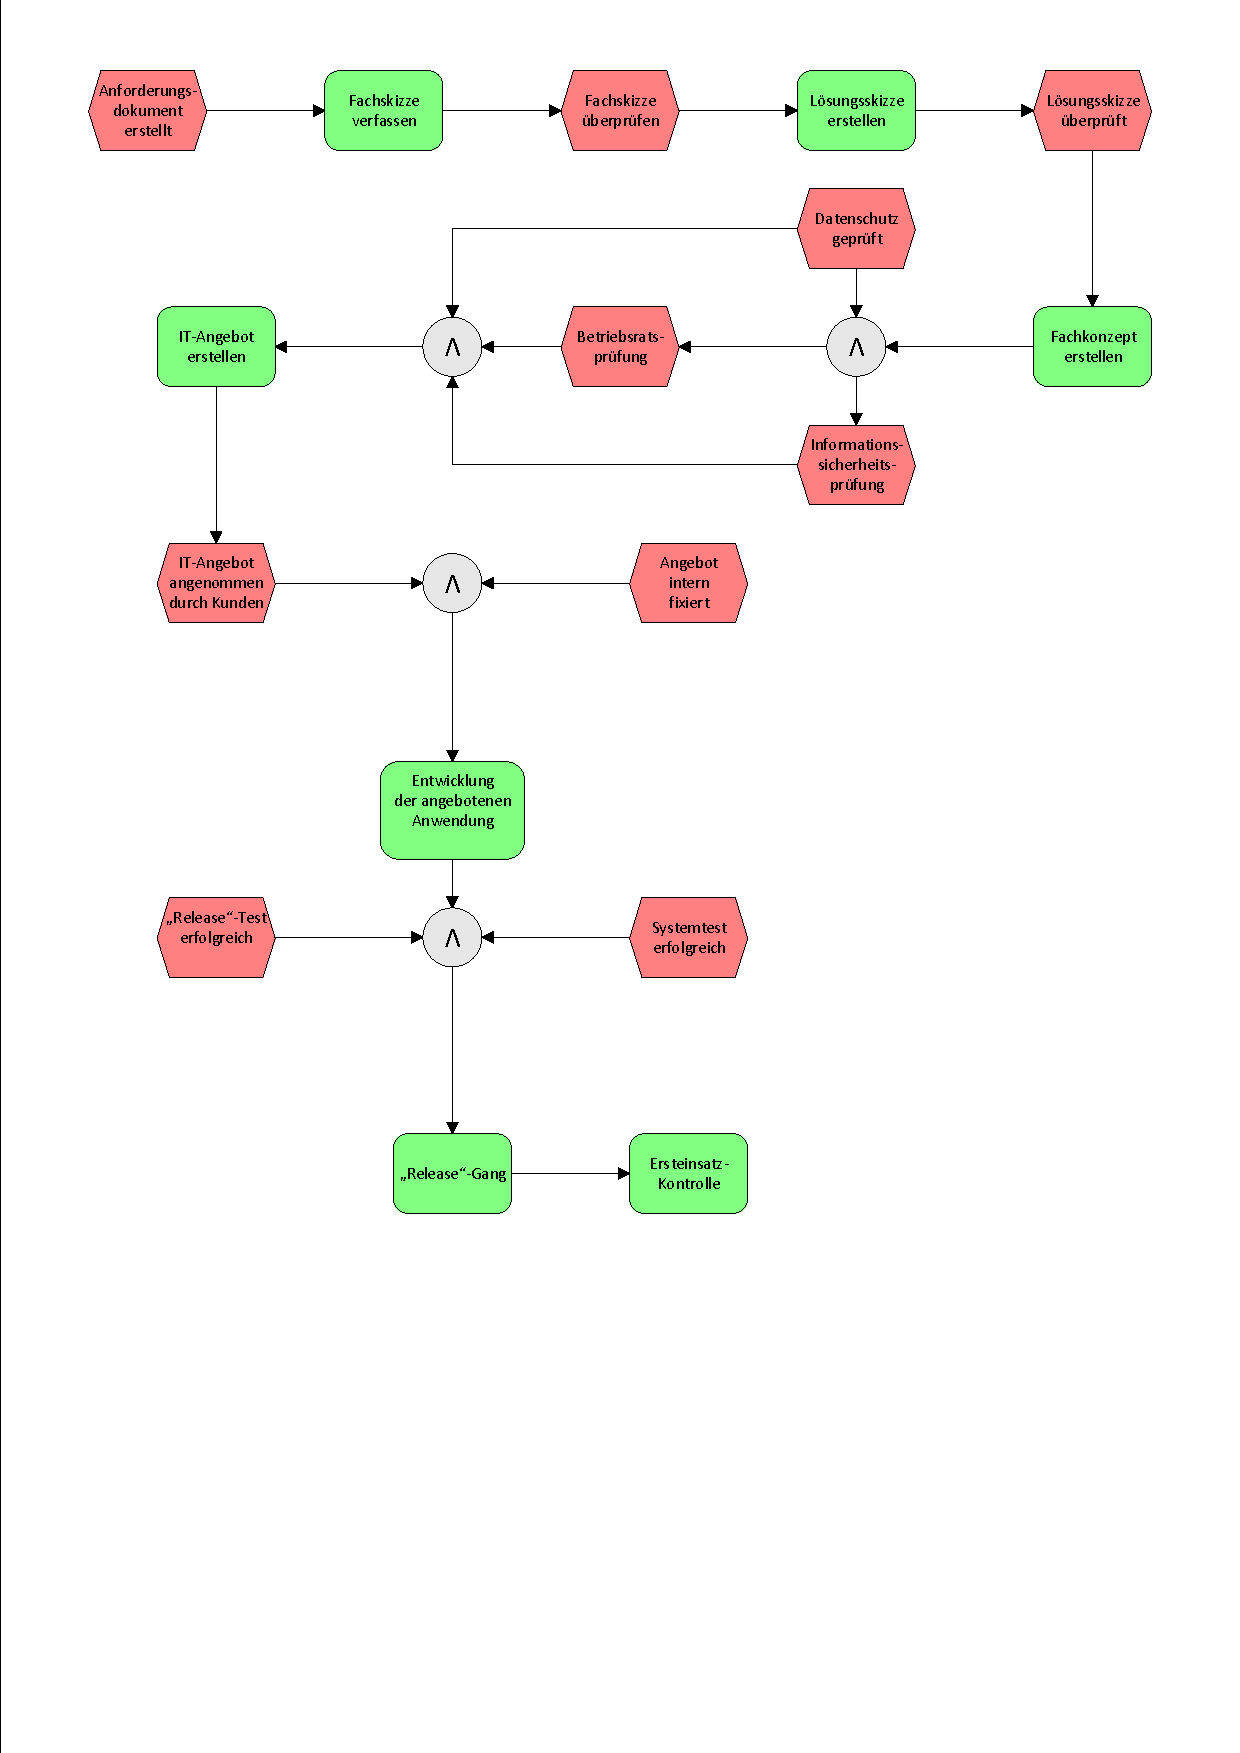
\includegraphics[scale=0.51]{img/prozessRelease.pdf}
	\caption{\acs{EPK} zum Geschäftsvorfall \enquote{Release}}
	\label{abb:meilensteineRelease}
	{\footnotesize Quelle: in Anlehnung an unternehmensinterne Dokumente}
	{\footnotesize \par \textit{unternehmensintern}}
\end{figure}

Die Abbildung \vref{abb:meilensteineRelease} zeigt die abgewandelte \ac{EPK} des Geschäftsprozesses: Die rot gefärbten Formen sind Ereignisse, die grünen Funktionen/Arbeitspakete und das grau gefärbte Symbol beschreibt eine logische \enquote{AND}-Verknüpfung. Dieser Prozess hat verschiedene Prüfstellen, die die Qualität der erstellten Dokumente überprüfen. Erst ab der Funktion \enquote{Entwicklung der angebotenen Anwendung} werden Anwendungen programmiert. Davor sind alle Aktivitäten zur Erstellung, Prüfung und Dokumentation der zu entwickelnden Anwendung durchzuführen. Diese sind mit erheblichen Aufwand verbunden: so muss die Kundin zusammen mit den Kundenmanagerinnen ein erstes Konzept entwickeln und beschreiben was das \enquote{statement of needs} ist. Dieses wird in den nächsten Schritten zu einem Anforderungsdokument überarbeitet, dabei werden auch mögliche Lösungsvorschläge berücksichtigt. Schließlich ist das Fachkonzepte und die Lösungsskizze erstellt. Die Kundenmanagerin kreiert ein IT-Angebot, dass der Kundin vorgelegt wird. Diese beiden Personenkreise verhandeln dann über die Kosten und Nutzen des Vorhabens. Sobald die Kundin zustimmt und alle anderen Zustimmungen (Betriebsrat, IT-Sicherheit und Datenschutz) eingeholt sind, startet die Entwicklung der beschriebenen Funktion. Nun folgend Tests in verschiedenen Umgebungen und dann die Freigabe für die Produktivsetzung der neuen Funktion/Anwendung. Danach prüft die Kundin, ob alle vorgesehenen Funktionen nach ihren Vorstellungen umgesetzt wurden. Dieses Vorgehen spiegelt einen linearen Vorgang wieder, der sich schwer an sich ständig veränderten Anforderungen anpassen kann. Ist das Fachkonzept freigegeben, kann an diesem nichts mehr geändert werden. Jedoch verändern sich die Anforderungen immer schneller und die Software hat einen immer kürzer andauernden Lebenszyklus innerhalb der \ac{SV}. Die Digitalisierung wird in der \ac{SV}-Strategie als zentraler Bestandteil beschrieben.\autocite[vgl.][]{sv_sparkassenversicherung_sv_2019} Somit wird die Forderung nach einer Anpassung des \enquote{Release}-Prozesses immer stärker.
\par
Durch die Veränderung des \enquote{Deployment}-Prozess ändert sich der gesamte \enquote{Release}-Prozess ebenfalls: So müssen die Planung und die Nicht-Anpassbarkeit des Fachkonzeptes überdacht werden. Außerdem ist der aktuelle Prozess, wie in Abbildung \vref{abb:meilensteineRelease} dargestellt, so mit den starren Regeln nicht mehr möglich. In einer Übergangsphase, bis ein neuer Geschäftsprozess entwickelt wurde, kann dieser aktuelle in einer abgewandelten Form benutzt werden. Diese Form müsste eine Änderung der Anforderungen und somit eine Änderung des Fachkonzeptes während der Entwicklung neuer Anwendungen zulassen. Dies kann zu inkonsistenten Daten in der Dokumentation führen und deswegen mit Vorsicht zu betrachten. Des Weiteren könnte eine Art Kategorisierung für die Anforderungen gemacht werden, d.\,h. zwingend umzusetzende Anforderung der Anwendungen wären ersichtlich. So könnten die Fachkonzepte in mindestens zu erfüllende und optimale Anteile unterteilt werden. 
\par
Die Container-Anwendungen unterstützen die Schnelligkeit der Entwicklung, da sie direkt mit einem entsprechenden \enquote{Deployment}-Prozess produktiv gehen können. Ist die Teststruktur automatisiert und die Dokumentationspflicht erfüllt, kann der Aufwand und damit die Kosten für die Entwicklung einer Funktion einer Anwendung beziehungsweise die Entwicklung einer kompletten Anwendung reduziert werden. Dies folgt aus der Tatsache, dass weniger Arbeitsstunden in die Betreuung, Entwicklung, Kontrolle und Dokumentation investiert werden müssen. Bleibt der Preis der Anwendung gleich, erhöht sich trotzdem der erziehlte Gewinn, da die Kosten sich reduzieren. Natürlich sind initial die Kosten höher, da die Entwicklung eines neuen Prozess sehr viel Aufwand darstellt.
\par
Momentan ist die \ac{SVI} in einer Übergangsphase, in der sie den Geschäftsprozess \vref{abb:meilensteineRelease} weiterhin nutzt. Jedoch wurden hier die oben genannten Veränderungen implementiert. Die illustrierte Weiterentwicklung des \enquote{Deployment}-Prozess (siehe Kapitel \vref{ff1}) ist eine Möglichkeit die Kosten durch Reduzierung des Betreuungsaufwandes in der Abteilung \ac{IE2} zu senken.

\section{\enquote{Business Case}: \enquote{Deployment} einer Container-Anwendung}
% TODO: IST-SOLL-Vergleich siehe Gliederung
Die \ac{SV} möchte verschiedene Prozesse dunkel verarbeiten, d.\,h. es soll keine/n Sachbearbeiter/in Arbeit mit der Erledigung dieser haben. Die Prozesse, die unter dem Namen \enquote{Meine \ac{SV}-Online Services} bekannt sind, sind auf der Webseite der \ac{SV}\footnote{unter \href{https://www.sparkassenversicherung.de/content/privatkunden/service/daten/index.html}{\enquote{Meine \ac{SV}-Online Services}}} zu finden. Dort können Kundinnen verschiedene Aufträge selbst durchführen, wie eine Rechnungs-/Policenkopie anfordern, ihre persönliche Daten ändern, einen Schaden melden, eine bestehende KFZ-Haftpflichtversicherung anpassen und eine Haftpflicht/Hausrat abschließen. Diese Prozesse sollten mittels \ac{BPMN} abgebildet werden. Ein \enquote{statement of needs} der \ac{SV} ist es, diese Prozesse selbstständig zu entwickeln. Durch diesen Wunsch entwickelte die \ac{SVI} in Zusammenarbeit mit der \ac{SV} eine Lösung. Es wurde ein Produktvergleich verschiedener Software-Hersteller durchgeführt. Schließlich hat sich die \ac{SV} in Zusammenarbeit mit der \ac{SVI} für die Software \textsc{Camunda} entschieden. Der Beschaffungsprozess wurde prozess-konform durchgeführt und die Entwicklungsarbeiten im Projektteam begannen. Die Anforderungen der Software \textsc{Camunda} beschrieben u.\,a., dass eine Container-Umgebung für die Verteilung dieser benötigt wird. Das Problem ist, dies war bei der Entscheidung zum Kauf der Software nicht berücksichtigt worden. Daraus resultiert die Anforderung, dass das \enquote{Deployment}-Team eine Lösung für die Verteilung von Container- und damit von \textsc{Camunda}-basierten Anwendungen erforscht und implementiert. Daraus folgt ein gemeinsames Projekt der Infrastruktur- und Betriebsabteilungen der \ac{SVI}: hier soll ein Software-Produkt gefunden werden, das revisions-konform und betriebstauglich ist. Die Kriterien der Revision werden von der \ac{BaFin}, sowie durch juristische Vorschriften und Gesetze bestimmt. Die Betriebstauglichkeit wird durch Anforderungen der jeweiligen Abteilungen beschrieben. Aus diesen Kriterien folgen Akzepttanzbestimmungen für das Software-Produkt, wie z.\,B. die Multi-Mandaten-Fähigkeit, die Integrationsbereitschaft zu \enquote{Cloud}-Plattform (\textsc{Amazon Webservices}, \textsc{Microsoft Azure}), die Isolationsfähigkeit der kompletten Plattform im Rechenzentrum, Verschlüsselung der Kommunikation und weitere. Mit Hilfe dieser Forderungen kann ein Produktvergleich durchgeführt werden zwischen den Lösungen von \textsc{Red Hat} (\textsc{OpenShift}) und \textsc{SuSe} (\textsc{CaaS}). Die Ergebnisse zeigten, dass der Hersteller \textsc{SuSe} zwei Produkte braucht, um die gegebenen Anforderungen zu erreichen. Im Gegensatz dazu erreicht \textsc{Red Hat} mit einem Produkt, \textsc{OpenShift}, alle Anforderungen der \ac{SVI}. Bei Betrachtung der zwei Produktlösungen sind keine nennenswerten Unterschiede zu erkennen. Die beiden Lösungen unterscheiden sich in den Kosten und, dass \textsc{SuSe} zwei Produkte für die Lösung benötigt. Die Kosten sind nachfolgend in der Tabelle \vref{tab:kostenvergleichProdukte} dargestellt. Schließlich wurde bedingt durch die lange Markterfahrung und die Nutzung durch andere Versicherungskonzerne die Lösung von \textsc{Red Hat} eingekauft. Die Lizenzkosten sind unter gewissen Annahmen getroffen, wie die Preise sind Listenpreise, die Berechnungsbasis sind \enquote{Cores} in einer Virtualisierungsumgebung u.\,Ä. Weitere Rechenzentrum-spezifische Details, wie die Ausstattung der Virtualisierungsserver und das Ausfallsicherungskonzept der \ac{SVI}, sind dementsprechend auch Annahmen zur Berechnung der Lizenzkosten.

\begin{table*}[h!]
	\centering
	\ra{1.3} %more space beetween rules
	
	\begin{tabular}{@{}lll@{}}\toprule[1.5pt]
		
		\textbf{Produkt} & \textbf{\enquote{Support}-Plan} & \textbf{Kosten} \\ \midrule
		% below rules with content
		\textsc{OpenShift} & Standard & 80 \enquote{Cores} $\widehat{=}$  86.400\,€ \\
		& & 160 \enquote{Cores} $\widehat{=}$  172.800\,€ \\
		
		\textsc{CaaS}\&\textsc{CaP} & Standard & 80 \enquote{Cores} $\widehat{=}$  80.000\,€ \\
		& & 80 \enquote{Cores} $\widehat{=}$  160.000\,€ \\
		
		\textsc{OpenShift} & Premium & 80 \enquote{Cores} $\widehat{=}$  128.000\,€ \\
		& & 160 \enquote{Cores} $\widehat{=}$  256.000\,€ \\
		
		\textsc{CaaS}\&\textsc{CaP} & Premium & 80 \enquote{Cores} $\widehat{=}$  111.200\,€ \\
		& & 80 \enquote{Cores} $\widehat{=}$  222.400\,€ \\		
		
		\bottomrule[1.5pt]
	\end{tabular}
	
	\caption{Vergleich der jährlichen Lizenzkosten}
	\label{tab:kostenvergleichProdukte}
	
\end{table*}
Durch Entscheidung der betreffenden Führungskräfte in Zusammenarbeit mit den Projektbeteiligten wird das Produkt \textsc{OpenShift} der Produktlösung von \textsc{SuSe} bevorzugt. Auch wenn, die Lizenzkosten und der initiale Einführungsaufwand höher sind als bei der \textsc{SuSe}-Lösung. Gemäß des oben genannten Vorgehens eines \enquote{Business case} (vgl. dazu Kapitel \vref{sec:businessCase}), muss bei einer Investition der Nutzen immer größer sein als die Kosten. Wenn das nicht gegeben ist, muss eine Abwägung getroffen werden, ob es trotzdem wirtschaftlich sinnvoll ist diese Investition zu tätigen. Hier sind die Akzeptanzkriterien nochmals zu überprüfen: \textsc{Red Hat} \textsc{OpenShift} ist bei der \ac{VKB} im Einsatz, die \ac{PNW} führt diese Anwendung aktuelle ein. Somit haben zwei andere öffentlich-rechtliche Versicherer diese Software im Einsatz. Auch die lange Markterfahrung von \textsc{Red Hat} im Bereich Finanzen und Automatisation sprechen für diesen Konzern. Im Gegensatz dazu ist die Produktlösung von \textsc{SuSe} noch nicht lange auf dem Markt (seit Herbst 2017) und die Lösung besteht zwei Produkten. Die Container-Anwendungen werden auf der Plattform \textsc{OpenShift} von \textsc{Red Hat} betrieben.
\par
Die vollständige \enquote{Business case}-Analyse wird teilweise durch die Projektkontrollgremien implementiert, so wird ein Kosten-Nutzen-Vergleich und eine Investitionsrechnungen durchgeführt. Jedoch wurde das Vorgehen auf die \ac{SVI} adaptiert. Dies ist der Unternehmensstruktur der \ac{SV} geschuldet: Die \ac{SV} ist unterteilt in sogenannte Ressorts. Die \ac{SVI} als Informatik-Dienstleitserin und vollständige Tochtergesellschaft ist dem Ressort drei \enquote{\textit{Leben/IT}} unter Dr.~Wittmann zugeordnet. Damit sind viele Tätigkeiten im \enquote{Controlling} Aufgabe der \ac{SV}, so auch die Verantwortung, wie Entscheidungen getroffen werden. 

\section{Ergebnis der Forschungsfrage zwei}
Die Ergebnisse der Forschungsfrage zwei -- Welche wirtschaftlichen Vorteile hat der Einsatz von Container auf den Prozess des automatisierten \enquote{Deployments}? -- werden nachfolgend kurz zusammengefasst. Eine kritische Betrachtung des gesamten Ergebnisses der Bachelorarbeit ist im Epilog (siehe Kapitel \vref{kritischeBetrachtung}) zu finden.

\paragraph{\enquote{Business Case}-Methodik} Keine richtige Methodik verwendet...

\paragraph{Probleme durch Entscheidungen der \ac{SV}} Die \ac{SV} hat weitreichende Entscheidung ohne die Berücksichtigung der aktuellen Infrastruktur ihrer Systeme gefällt.